\documentclass[sigconf]{acmart}

% A4 instead of letter paper
\geometry{a4paper}

\usepackage[babelshorthands]{polyglossia}
\setdefaultlanguage[babelshorthands=true]{german}
\usepackage[autostyle=true, german=quotes]{csquotes}
\usepackage{booktabs} % More formal table style.
\usepackage{xcolor}

% ACM style ``tweaking''
\settopmatter{printacmref=false}                   % Removes citation information below abstract
\renewcommand\footnotetextcopyrightpermission[1]{} % Removes footnote with conference information in first column
\pagestyle{plain}                                  % Removes running headers

% Code
\definecolor{light-gray}{gray}{0.95}
\newcommand{\code}[1]{\colorbox{light-gray}{\texttt{#1}}}

% Figures
%\DeclareGraphicsRule{.ai}{pdf}{*}{}% Handle .ai files as .pdf files.
%\DeclareGraphicsExtensions{.pdf,.ai,.jpg,.png}
%\pdfpagebox 5% Use ArtBox instead MediaBox. 1=MediaBox, 2=CropBox, 3=BleedBox, 4=TrimBox, 5=ArtBox. (shell: pdfinfo -box <pdf-file>)
%\setkeys{Gin}{pagebox=artbox}% Alternative (necessary for newer tex versions) for \pdfpagebox 5 in preceding line.
\graphicspath{{../report-ufo-figures/}}

%\usepackage[backend=biber]{biblatex}
%\addbibresource{report-ufo.bib}


\usepackage[math]{blindtext} % TODO Remove after adding own content.
\usepackage{hyperref}

\begin{document}

\title{Report of Group FOOBAR}
\subtitle{Maybe a longer but still short subtitle.}         % Optional.

\keywords{Übung {\glqq Big Data Analytics\grqq}, Sommersemester 20XX}

\author{Erika Musterfrau}
\affiliation{%
    \institution{%
        Martin-Luther-Universität Halle-Wittenberg
    }
}
\email{erika.musterfrau@student.uni-halle.de}

\begin{abstract}
 Some general hints on what to mention in an abstract: What are the questions you address? Why are they interesting? What approaches did you use? What answers did you find?
 
 As for how to structure the abstract: Give some motivation and context on the general topic you address (1--2~sentences). Then state the specific questions you address (1--2~sentences) and describe how you approach them (2--3~sentences). Finally, results and some conclusion (1--3~sentences).
\end{abstract}

\maketitle

\section{Introduction} \label{introduction}

The abstract in more detail: Tell the whole story, from context to conclusion \ldots\ still high-level but with target audience of computer scientists. Maybe you want to reference some publication, just give the authors of some publication, or give the authors and the reference. Including graphics also is usually dead simple, like with Figure\ref{rubber-duck}.

\begin{figure}[t]
    \centering
    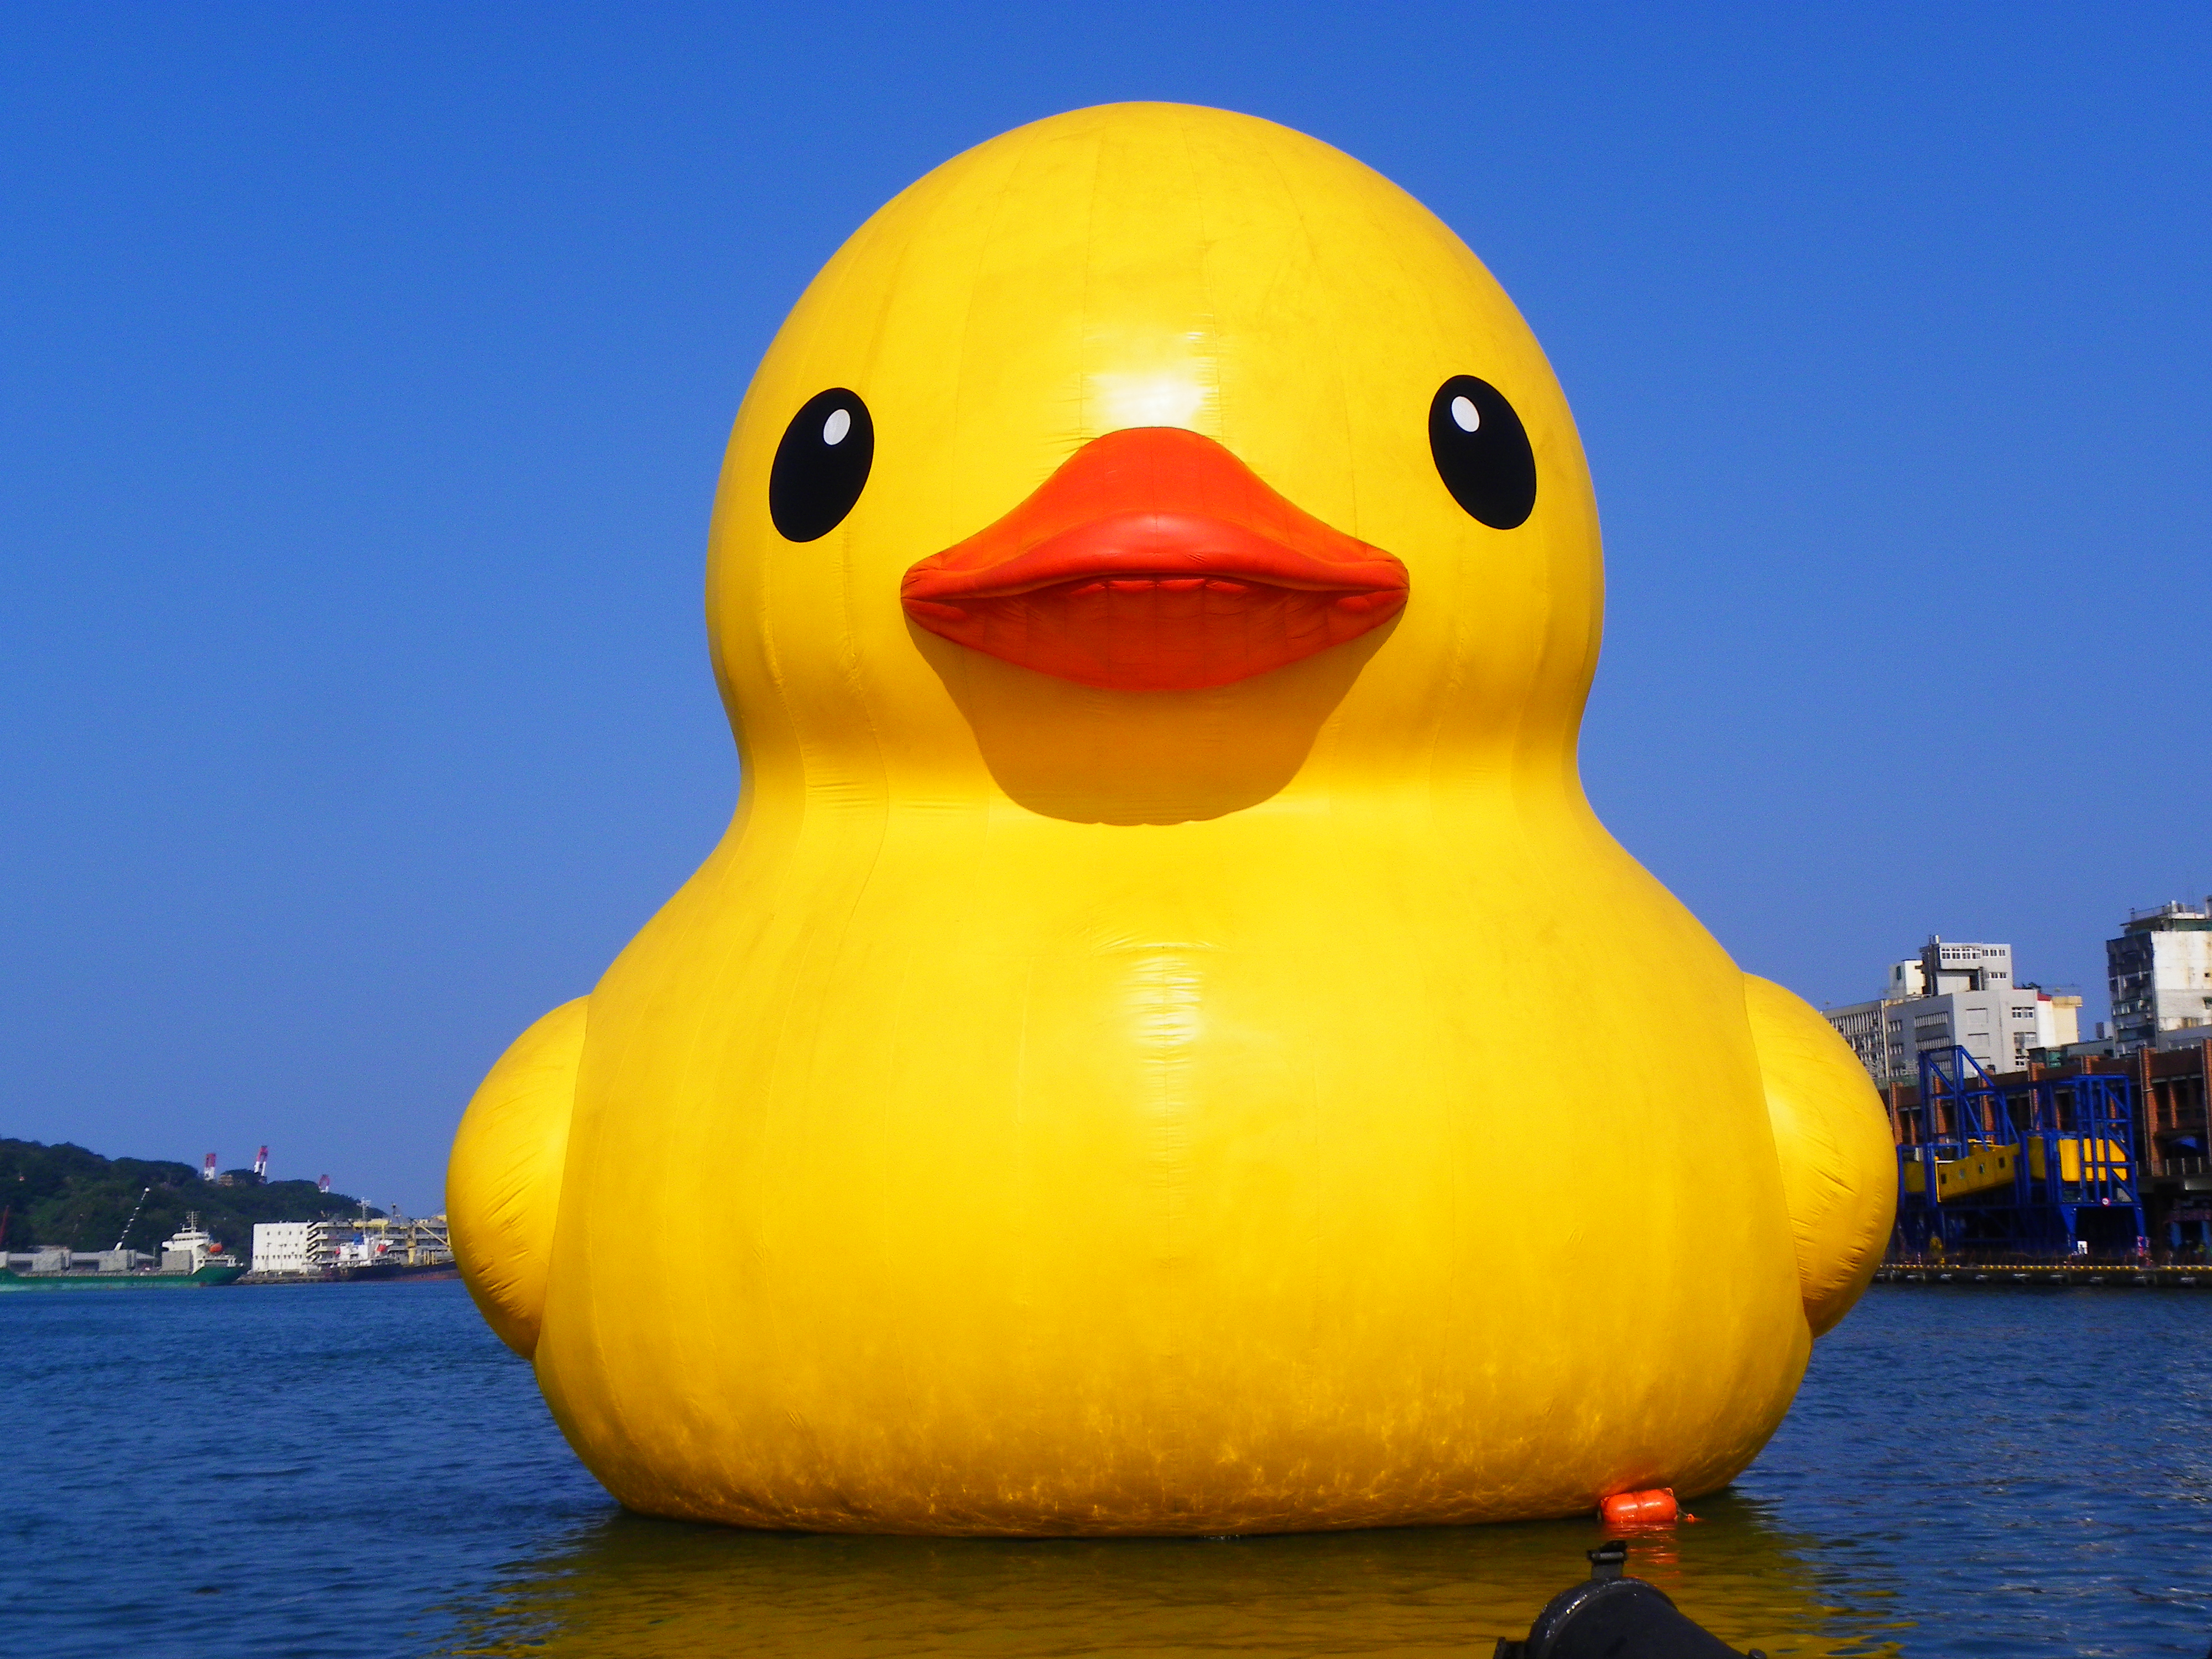
\includegraphics[width=\columnwidth]{rubber-duck}
    \caption{Some large rubber duck.}
    \label{rubber-duck}
\end{figure}


\section{Daten} \label{data}

Die verwendeten Datensätze stammen aus einer Datenbank vom \enquote{National UFO Reporting Center} (NUFORC). In diese Datenbank kann jede Person ihre vermeintliche Ufo-Sichtung -- entweder online über ein Formular oder per Telefon -- eintragen. Des Weiteren senden gewisse Messstationen (z.B. MADAR Nodes) auffällige Messdaten automatisch an die Datenbank. Um offensichtlichen Fakes entgegenzuwirken werden die eingereichten Daten vor der monatlichen Veröffentlichung von den Betreibern des Portals überprüft.

Jeder Eintrag des Datensatzes besteht aus dem Datum und der Uhrzeit der Sichtung, der Stadt sowie dem Kürzel des dazugehörigen Bundesstaates (ausschließlich für die USA), einer klassifizierten Beschreibung der Form des Ufos und gegebenenfalls einer kurzes Zusammenfassung und Beschreibung aus der Sicht des Einsenders.

Für diese Daten haben wir eine einfache Datenbank erstellt, um auch offline auf diese zugreifen zu können. Um die Daten einfacher verarbeiten zu können, bereiten wir diese während der Abfrage von unserer Datenbank auf und treffen eine Vorauswahl an brauchbaren Daten. Die Kriterien für die Vorauswahl wurden durch stichprobenartige Abfragen festgelegt. Dem entsprechend werden Einträge von vorhin beschriebenen externen Messstationen, Einträge mit fehlenden Inhalten oder \enquote{?} als Inhalt nicht betrachtet. Der Datentyp aller Attribute ist der Einfachheit halber nur string. Zu einem späteren Zeitpunkt werden Datum und Uhrzeit in ein datetime-Format überführt. Mit dem Wissen aus den stichprobenartigen Abfragen legen wir und auf die zwei gängigsten Formate fest -- 'm/d/y H:M' und 'm/d/y'. Andere in dem Datensatz vorkommenden Formate oder von den Einsendern eigenständige Angaben beachten wir nicht. Die aufbereiteten Daten werden letztendlich durch das Tripel \code{datetime}, \code{city} und \code{state} beschrieben.

Als Quelle für die Wetterdaten haben wir uns letztendlich für \enquote{Meteostat}(Link) entschieden. Auf diese Daten wird über die dazugehörige Python-Library zugegriffen. Essenziell für unser Projekt sind die Attribute \code{tsun} (Anzahl der Sonnenminuten) und \code{coco} (Klassifizierter Zustand des Himmels). Die Daten sind für unsere Vorhanben bereits eine ausreichende Qualität, sodass in diesem Fall keine weitere Aufbereitung und Säuberung der Daten nötig ist.

\begin{table}[t]
    \caption{Kennzahlen des Datensatzes.}
    \label{tab:data}
    \centering
    \small
    \begin{tabular}{l r}
        \toprule
        Einträge & Anzahl\\
        \midrule
        Gesamt & 96~924\\
        Davon einzigartige Orte & 25~234\\
        \midrule
        Orte mit Wetterdaten, gesamt & 2~020\\
        Davon mit Sonnenminuten pro Stunde & 26\\
        Davon mit Sonnenminuten pro Tag & 116\\
        Davon mit condition codes & 1~886\\
        \bottomrule
    \end{tabular}
\end{table}
\section{Research Question 1} \label{question1}  % Change title accordingly

Describe how you worked on the first question you address.

\blindtext

\section{Forschungsfrage} \label{forschungsfrage} % Change title accordingly

Describe how you worked on the second question you address.

\blindtext

\section{Evaluation} \label{evaluation}

Die Bearbeitung der Forschungsfrage hat folgende Ergebnisse hervorgebracht: Aus ursprünglich 96~924 potenziell relevanten Ufo-Sichtungen im Datensatz konnten für 2~020 Sichtungen zu dem Zeitpunkt passende Wetterdaten gefunden werden, das entspricht ungefähr 2,1\%. Mit welcher Art der drei Vergleichsdaten die Sichtungen analysiert wurden lässt sich in Tabelle \ref{tab:data} ablesen.

\begin{figure}[t]
    \centering
    \includegraphics[width=\columnwidth]{hourly_suntime_boxplot}
    \caption{Sonnenminuten pro Stunde.}
    \label{fig:hourly_suntime}
\end{figure}

Die Vergleichsdaten mit dem am Abstand wenigsten Vorkommen bilden die Sonnenminuten pro Stunde mit lediglich 26 Einträgen. Wie in Abbildung \ref{fig:hourly_suntime} zu erkennen ist, befindet sich die Mehrheit davon im Bereich von 0 bis 5 Sonnenminuten pro Stunde. Vereinzelte Ausreißer reichen gegen 50 bis 60 Sonnenminuten.%Aufgrund der sehr geringen Datenmenge und der Erkenntnis, dass es sich bei fast allen Werten um \enquote{0 Minuten} handelt,  

\begin{figure}[t]
    \centering
    \includegraphics[width=\columnwidth]{daily_suntime_boxplot}
    \caption{Sonnenminuten pro Tag.}
    \label{fig:daily_suntime}
\end{figure}

Abbildung \ref{fig:daily_suntime} beschreibt die Verteilung der Sonnenminuten pro Tag an jeder verfügbaren Ufo-Sichtung. Die mittleren 50\% der Ergebnisse sind hierbei, im Gegensatz zu den stündlichen Sonnenminuten, breiter verteilt. Sie reichen von 200 bis 700 Sonnenminuten pro Tag mit wenigen Ausreißern, welche nur gegen weniger Minuten streben. Im Schnitt scheint die Sonne während eines Tages, an dem ein vermeintliches Ufo gesichtet wurde, um die 500 Minuten -- also etwas mehr als 8 Stunden. In Anbetracht dessen, dass die durchschnittlichen Sonnenstunden in den USA im Bereich zwischen 2 Stunden im Winter und bis zu 12 Stunden im Sommer reichen, kann man den Ufo-Sichtungen eine leichte Überdurchschnittlichkeit an Sonnenstunden zuordnen\cite{statista:2021}.

\begin{table}[t]
    \caption{Condition Codes.}
    \label{tab:coco}
    \centering
    \small
    \begin{tabular}{l l r}
        \toprule
        Code & Weather Condition\cite{coco:2021} & Anzahl\\
        \midrule
        0 & - & 15\\
        1 & Clear & 227\\
        2 & Fair & 603\\
        3 & Cloudy & 363\\
        4 & Overcast & 93\\
        5 & Fog & 186\\
        7 & Light Rain & 219\\
        8 & Rain & 51\\
        9 & Heavy Rain & 9\\
        12 & Sleet & 1\\
        14 & Light Snowfall & 42\\
        15 & Snowfall & 2\\
        16 & Heavy Snowfall & 1\\
        17 & Rain Shower & 9\\
        18 & Heavy Rain Shower & 23\\
        25 & Thunderstorm & 35\\
        26 & Heavy Thunderstorm & 5\\
        27 & Storm & 2\\
        \bottomrule
    \end{tabular}
\end{table}

\section{Fazit} \label{fazit}

Den Ergebnissen aus Kapitel \ref{evaluation} ist zu entnehmen, dass es, in Hinblick auf die verwendeten Vergleichdaten, bei vermeintlich besserem Wetter mehr Ufo-Sichtungen gemeldet werden als bei schlechterem Wetter. Da allerdings nur für eine sehr geringe Anzahl an Ufo-Sichtungen dazu passende Wetterdaten gefunden wurden, lässt sich die Aussagekraft der Ergebnisse nicht als endgültiges Ergebnis festlegen, sondern kann als Wegweiser für weitere Forschungen dienen. Eine weiterführende Herangehensweise wäre zum Beispiel die Betrachtung Wetterdaten von anderen Anbietern. Für Forschungen, welche außerhalb der Wetterzusammenhänge liegen, erweisen sich Uhrzeit der Sichtung (Morning Morality Effekt) sowie die Frage, ob es in der Nähe von Weltraumbahnhöfen, militärischen Einrichtungen oder Flughäfen zu überdurchschnittlich vielen Sichtungen kommt, als interessant. Ob es sich bei den vermeintlichen Ufo-Sichtungen wirklich um Ufos handelt, oder diese \enquote{Sichtungen} nur Verwechselungen mit anderen Flugobjekten oder bewusste Fehlinformationen sind, können allein durch die verwendeten Daten nicht belegt werden.

\begin{figure}[t]
    \centering
    \includegraphics[width=\columnwidth]{condition_codes_pie.png}
    \caption{Verteilung der Condition Codes.}
    \label{fig:coco_pie}
\end{figure}

%\bibliographystyle{ACM-Reference-Format}
%\printbibliography

\end{document}
